%%%%%%%%%%%%%%%%%%%%%%%%%%%%%%%%%%%%%%%%%%%%%%%%%%%%%%%%%%%%%%%%%%%%%%%%
% RevTeX 4.1 LaTeX
% Kevin C. Young
% Scalable & Secure Systems Research (08961)
% Thu Mar  5 15:29:19 PST 2015
%%%%%%%%%%%%%%%%%%%%%%%%%%%%%%%%%%%%%%%%%%%%%%%%%%%%%%%%%%%%%%%%%%%%%%%%

\documentclass[aps,nofootinbib,pra,notitlepage,twocolumn]{revtex4-1}

\usepackage{amsfonts,amsmath,amssymb,amsthm}
\usepackage{array,bm,color}
\usepackage{epsfig,graphicx,nomencl,revsymb4-1,upgreek,url}
\usepackage{hyperref}
\usepackage{algorithm}
\usepackage{algpseudocode}
\usepackage{graphicx}
% \usepackage[justification=justified,font=small]{caption}
\graphicspath{{./figures/}}
\hypersetup{colorlinks=true, pdfauthor=Kevin C. Young, pdftitle=Decorrelating Errors}
\newcommand{\tr}{{\rm Tr\thinspace}}
\newcommand{\bra}[1]{\ensuremath{\left\langle{#1}\right\vert}}
\newcommand{\ket}[1]{\ensuremath{\left\vert{#1}\right\rangle}}
\newcommand{\braket}[2]{\left\langle #1 | #2 \right\rangle}
\newcommand{\ketbra}[2]{\left| #1 \right\rangle\!\!\!\,\left\langle #2 \right|}
\newcommand{\abs}[1]{\left\vert #1 \right\vert}
\newcommand{\expect}[1]{\ensuremath{\left\langle{#1}\right\rangle}}
\newcommand{\timeorder}{\ensuremath{\underset{\leftarrow}{\mathcal{T}}}}
\newcommand{\ident}{{\mathbb1}}
\newcommand{\order}[1]{\mathcal{O}\left( #1 \right)}
\newcommand{\diag}[1]{\mathrm{diag}\{#1\}}
\newcommand{\trans}[1]{#1^\mathsf{T}}
\newcommand{\T}{\mathsf{T}}

\newcommand{\erf}[1]{Eq.~(\ref{#1})}
\newcommand{\needcite}{{\color{blue}\textsuperscript{[citation needed]}}}
\newcommand{\note}[1]{{\color{red}[#1]}}
\newcommand{\kcy}[1]{{\color{red}[#1]_{\rm{KCY}}}}
\newcommand{\amp}[1]{{\color{red}[#1]_{\rm{AMP}}}}
\setlength{\jot}{10pt}
%-------------Header begins here----------------------------------------
\begin{document}
% \tableofcontents
\title{Decorrelating Errors in Quantum Gates by Random Gate Synthesis - A BOCS of Control Solutions}

\author{Anthony Polloreno}
\email[Email: ]{anthony@rigetti.com}
\affiliation{Rigetti Computing, Berkeley, CA}

\author{Kevin C. Young}
% \email[Corresponding author: ]{kyoung@sandia.gov}
\affiliation{Sandia National Laboratories, Livermore, CA}

\date{\today}

\begin{abstract}
Thresholds for fault-tolerant quantum computation are often calculated assuming a noise model in which errors are uncorrelated. While convenient for simulation, these error models are often unphysical. Work by Preskill and others has shown that arbitrarily long computations may be performed even in the presence of spatial and temporal correlation, provided the correlation is sufficiently weak and decays sufficiently quickly, but at the cost of a significantly lower threshold. The success of algebraic decorrelation methods, such as dynamical decoupling, demonstrate that quantum control techniques are capable of reducing noise correlations. We propose to introduce similar methods at the gate synthesis level to effect the decorrelation of errors in quantum circuits, thereby increasing the threshold for fault-tolerant computation in such systems. We show numerically and experimentally on a superconducting qubit that these methods can reduce the magnitude of the diamond norm of the error by at least an order of magnitude.
\end{abstract}

\pacs{}

\maketitle

\section{Introduction}

Steady progress has been made in the theory of quantum error correction, proving higher thresholds for increasingly general models of noise \cite{Aharonov2006, 1609.00510, https://doi.org/10.7907/z96m34sc, Kubica2018, Wang2003, Campbell2017}. These results show that quantum computation is feasible in principle, however recent NISQ \cite{Preskill2018} devices have noise that is not only often above thresholds, but that also violates fundamental assumptions made by the models used in these results, such as Markovianity \cite{Kitaev1997} and independence of errors\cite{Knill1998}. With these assumptions violated, many properties of system performance and correctness can no longer be guaranteed.

To make matters worse, the ways in which a quantum computer can fail to meet these assumptions are manifold\cite{Kelly2018, BlumeKohout2017, Klimov2018}, and even when the noise is Markovian, many models and existing work make strong simplifying assumptions about the structure of the noise. As an example, Pauli channels are often used to model systems due to their classical simulability\cite{quant-ph/9807006}, even in the absence of physical motivation\cite{Aliferis2007, Knill2005, Wang2011, DuclosCianci2010, Wootton2012, Bombin2012, Puzzuoli2014, aliferis2008accuracy}. Because of this, a common approach is to attempt to use those thresholds to give a loose lower bound for thresholds with lower noise\cite{Puzzuoli2014}. This approach is correct and rigorous, but produces overly-pessimistic bounds on device performance.

Relatedly, many characterization routines assume that the noise is well-behaved so that they can make non-trivial assertions about performance. If these assumptions are violated, the utility of many of these algorithms is drastically reduced. For example, randomized benchmarking and tomography will report incorrect answers without any syndrome in the case of non-Markovian noise \cite{Merkel2013}. Slightly more helpful, gate-set tomography will report that the gateset failed to be Markovian, however figuring out how to bring it back to the space of the Markovianity can be challenging.

<<<<<<< HEAD
Other authors have considering the problem of coherent error at the logical gate level, considering over rotations that might arise from gate approximation \cite{Campbell2017, 1612.01011}, and others have considered methods of \textit{twirling} error, such that it turns into a Pauli channel through random compilation methods\cite{Wallman2016, Ware2018}.
=======
Many authors have approached these problems at varying levels of abstraction, each with their own benefits and short-comings. At the level of unitary synthesis, authors have considered randomizing over errors that might arise from gate approximations like Solovay-Kitaev \cite{Campbell2017, 1612.01011}. While this affords the ability to prove theorems that guarantee quadratic improvements to performance, they do not offer routines which are accessible and implementable with current coherence times. At the level of compilation, Frame Randomization\cite{Wallman2016, Ware2018}can be used to average over noise by \textit{twirling} error over an appropriately selected unitary 2-design.\cite{roy2009unitary} This has the advantage of being implementable\cite{Ware2018}, but it can require intensive use of classical resources, such as precompilation and generation of many waveform variants, and becomes more difficult when the gates being used are not in the Clifford group, as is the case in various quantum computing architectures. The general theme of these results is that of randomized decoupling\cite{Viola2005, Viola}. By introducing classical randomness into quantum computations, both coherent and non-Markovian can be transformed to incoherent, independent, Markovian noise, to varying degrees. In this paper, we explore a different method of solving these problems. We propose to inject additional decorrelating randomness into the system during physical gate synthesis through the use of \emph{balanced optimal control solutions} (BOCSs).
>>>>>>> 389689a795ed459047e293f4429031af7ef1b0c8

\begin{figure}
  \centering
  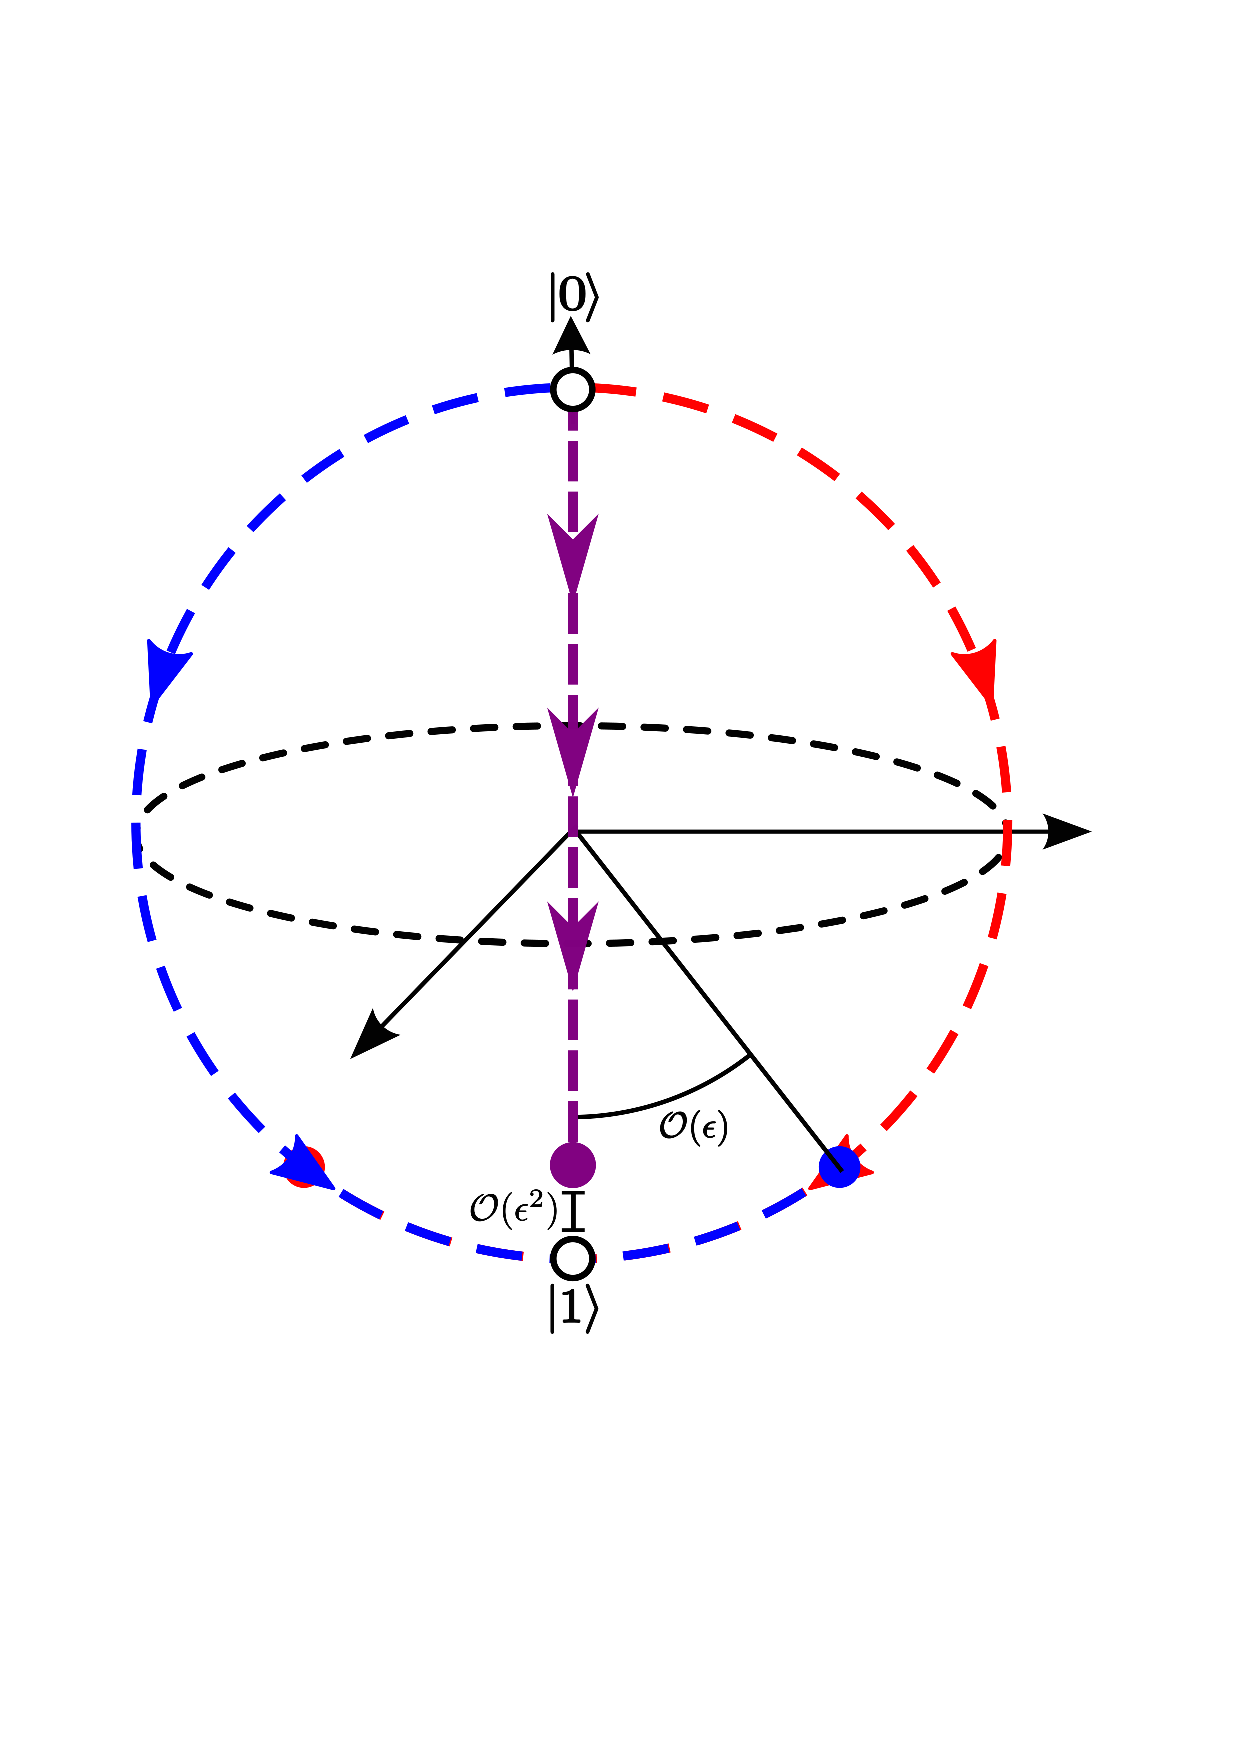
\includegraphics[width=\columnwidth]{simple_example.pdf}
  \caption{An example of a balanced control solution. Using optimal control, two implementations of a $Z_\pi$ gate are designed to have equal and opposite sensitivity to errors (if one implementation over-rotates by angle $\theta$, then the other \emph{under}-rotates by $\theta$). Each time the gate is used, one of these implementations is chosen at random. The resulting quantum channel is equivalent to a perfect implementation of the gate followed by dephasing of $\order{\theta^2}$.}
  \label{fig:simple_example}
\end{figure}

\section{Theory}
 BOCSs are families of control solutions, $c_i(t)$, where each member of the family approximates the same target gate with slightly different errors, for any given instance a noise Hamiltonian. That is, for a target unitary operator $U_T$, we seek a family of approximating $U_i = \mathcal{T}e^{-i\int c_i(t)H(t, \delta)}$ to the target gate, such that the family of unitary approximations is \emph{balanced}. A balanced family is one which satisfies, for some small $\alpha$,
\begin{equation}\label{eq:1}
  \frac{1}{N}\sum_{i=1}^N \omega_i U_i \rho U_i^\dagger = DPN[\alpha]\left(U_T \rho U_T^\dagger \right)
\end{equation}

where $DPN[\alpha](\rho)$ is a \textit{generalized} depolarizing noise channel with strength $\alpha$. (For the rest of this paper, we will refer to them as just depolarizing channels.) Such a channel is defined as:
\begin{equation}\label{eq:2}
  DPN[\alpha](\rho) \rightarrow (1-\alpha)\rho + \alpha\sum p_i \sigma_i\rho\sigma_i
\end{equation}
with $p_i$ summing to one. This means that a for a family of controls that are a BOCS, there exists a weighting $p_i$, such that when the unitary approximations are averaged over with that weighting, they implement the target unitary followed by a depolarizing channel.

<<<<<<< HEAD
Because BCSs produce error channels that are depolarizing, correlations in the noise are reduced, and by generating controls that produce BCSs over a range of parameter values, a system can be made less sensitive to non-Markovian errors, e.g. drift. In addition, we will give numerical results showing that the fidelity of the new approximation to $U$ is not much worse than the fidelities of the constituent controls.

\section{A Simple Example}
As a somewhat trivial example, consider a single-qubit $X_\pi$ gate. We will assume that the control hardware implementing this gate is slightly miscalibrated, leading to an over-rotation by angle $\theta$. The diamond distance between this channel and the ideal implementation is $\theta$. If the gate were repeated $N$ total times, the target qubit would experience an accumulated over-rotation of $N\theta$. As shown in Fig.~\ref{fig:simple_example}, a balanced implementation of this gate may consist of two implimentations: 1) the original $X_\theta = \exp(-i (\pi/2+\theta)\sigma_x)$ and 2) the conjugate $X_\theta^\dagger = \exp(-i (\pi/2+\theta)\sigma_x)$. Each time the gate is required in a quantum circuit, one member of this balanced set is chosen uniformly at random. After $N$ applications of this gate, the mean over-rotation angle is zero, with a standard deviation of $\sqrt{N}\theta$. This is equivalent to the perfect gate followed by a stochastic Pauli $X$ error with rate $\theta^2$. The diamond norm of the channel is $\theta^2$, This has the effect of decreasing the norm of the noise channel and decorrelating the over-rotation error (Figure \ref{fig:simple_example}). In this simple example, we can solve the minimization problem given by equation \ref{eq:minimization} analytically. In particular, if we choose the weights in \ref{eq:1} such that $\omega_i=1$, and we choose to represent our gates in the vectorized superoperator representation, then:
=======
Thus, one property of BOCSs is that if each approximation of the target gate is correct to within $\epsilon$ in operator norm and $\alpha\leq\epsilon^2$, then the diamond distance of the BOCS to $U_T$ is also no larger than $\epsilon^2$. This follows from the mixing lemma proven by Campbell and Hastings in \cite{Campbell2017} and \cite{1612.01011}, and tells us that we can lower bound the worst case performance of a BOCS by the square of the error on each member of the BOCS, and linearly in the error of the weighted average. Because a set of parameters always exist that result in quadratically smaller error, it is then clear that in priniple BOCSs can always quadratically decrease the error in our approximation (in diamond norm). Moreover, in the setting where our system's performance is non-Markovian, e.g. drift, optimizing our BOCSs over a range of control parameters can reduce the non-Markovianity of the noise. As the name suggests, the task of generating BOCSs in this paper will fall to optimal control. 

\section{A Simple Example}
As a somewhat trivial example, consider a single-qubit rotation-angle error, such as from stochastic laser amplitude fluctuations. A BOCS may consist of an $X_\pi$ pulse, as well as an $X_{-\pi}$ pulse (i.e., a clockwise and counter clockwise rotation of the qubit). In the case of excess amplitude, the $X_\pi$ pulse will result in an over-rotation error, while the $X_{-\pi}$ pulse will result in an \emph{under}-rotation error. When it comes time to perform the target gate in a quantum circuit, one member of the BOCS is chosen uniformly at random. This has the effect of decreasing the norm of the noise channel and decorrelating the over-rotation error (Figure \ref{fig:simple_example}). In this simple example, we can analytically find a solution to Equation \ref{eq:1}. Specifically, by choosing weights $\omega_i=1$, we see:
>>>>>>> 389689a795ed459047e293f4429031af7ef1b0c8

\begin{equation}
  \begin{gathered}
    \frac{1}{2}(X^*_{\pi + \epsilon}\otimes X_{\pi + \epsilon} + X^*_{-(\pi + \epsilon)}\otimes X_{-(\pi + \epsilon})) \\
    = (\sin^2{\frac{\pi + \epsilon}{2}}I\otimes I + \cos^2{\frac{\pi + \epsilon}{2}}X\otimes X)X\otimes X \\
    \approx DPN[\epsilon^2]X\otimes X
  \end{gathered}
\end{equation}

Therefore, for a rotational error of angle $\epsilon > 0$, we see that $X_\pi$ and  $X_{-\pi}$  form a BOCS, with $\alpha\approx\epsilon^2$.



\section{Optimal Control Problems}\label{ocp}
\subsection{Random Gate Synthesis}
Generating BOCSs can be done in a variety of ways, using any  of the many available quantum optimal control techniques \cite{Khaneja2005, Caneva2011, Machnes2018}. For our numerics, we chose to use the GRAPE algorithm to generate candidate pulseshapes to approximate the target gate. First described in \cite{Khaneja2005}, the GRAPE (GRadient Ascent Pulse Engineering) algorithm is a technique for finding piecewise constant control sequences that approximate a desired unitary, $U_T$. Defining our uncontrolled Hamiltonian as $H_0$, our control Hamiltonians as $H_{i\neq 0}$, and our \textit{control matrix} $c_{ij}$ as containing control amplitude associated with the $i^{th}$ time step and the $j^{th}$ hamiltonian, we can write our approximate unitary at any timestep as
\begin{equation}\label{eq:3}
  U_i = \exp\{-i\Delta t(H_0 + \sum_{j=1}^{n}c_{ij}H_{j}\}
\end{equation}
Then, to measure the simularity of our approxiate unitary $U_n$ to our target unitary $U_T$, we can define a cost function $J(U) = Tr\{U_T^{\dagger}U_n\}$.

To optimize this cost function we can perform the following standard update loop for some threshold value $\varepsilon > 0$ and step size $\delta > 0$:
\begin{algorithm}[H]
\floatname{algorithm}
  \caption{\textsc{\textbf{Gradient Ascent}}}
  \begin{algorithmic}
    \While{$J(U_n) < (1-\varepsilon$)}
    \State $c_{ij} \rightarrow c_{ij} + \delta\frac{\partial J(U)}{\partial c_{ij}}$
    \For{$1 \leq i \leq n$}
    \State $U_i \rightarrow \exp\{-i\Delta t(H_0 + \sum_{i=0}^{n}c_{ij}H_j)\}$
    \EndFor
    \State $U \rightarrow \prod_{i=1}^nU_i$
    \EndWhile
  \end{algorithmic}
\end{algorithm}

In general these gradients can be computed by propagating partial derivatives of the cost function with respect to control parameters through each timestep of the  via the chain rule. However, in \cite{Khaneja2005} Khaneja et al. derive a simple update formula that is correct to first order. In particular one can show that:
\begin{equation}\label{eq:update}
  \begin{split}
\frac{\partial J(U)}{\partial u_{ij}} = -2Re\{\braket{{U_{j+1}^{\dagger}...U_N^{\dagger} U_T}}{i\Delta tH_jU_j...U_1}\\
\braket{U_j...U_1}{U_{j+1}^{\dagger}...U_N^{\dagger} U_T}\} +  \mathcal{O}(\Delta t^2)
  \end{split}
\end{equation}


In our numerical results in Section \ref{1Q Gates} and \ref{2Q Gates}, we consider the controls to have quasi-static Gaussian distributed errors, so to generate controls that are robust drift in these controls we modify our gradient to instead be:
\begin{align}\label{quadrature}
\frac{\partial \tilde J(U)}{\partial u_{ij}} =
\int p(\vec{\delta})\frac{\partial J(U(\vec{\delta}))}{\partial u_{ij}} d\vec{\delta}
\end{align}
with $p(\vec{\delta})$ Gaussian distributed, as has been done in previous works \cite{Goerz2014} to ensure that the optimal control results are robust over a wide range of errors. To make this averaging tractable, we approximate this integral using Gaussian quadrature, approximating the cost functions as a low order polynomial. 

Concretely, we consider a Hamiltonian of the following form:
\begin{equation}\label{eq:2}
  H(t) = \delta_0H_0 + \sum_{i=1}^n (1 + \delta_i)c_i(t)H_i
\end{equation}
for control Hamiltonians $H_i$, free evolution Hamiltonian $H_0$ and random variables $\delta_i$, that model some small uncertainty in parameters in the Hamiltonian. Such a model might describe a superconducting qubit quantum processor where control amplitudes for the RF pulses vary over time, or a trapped ion quantum computer where the intensity, frequency, or phase of the laser might drift over time\cite{Kelly2018, Lekitsch2017}. Correlations between different $\delta_i$ might arise, for instance, if two of the controls have the same noise source, e.g. $RX$ and $RY$ gates in superconducting qubit architectures might use the same AWG and pulse envelope, and suffer from the same diurnal temperature drift of control electronics.



\subsection{BOCS Approximation}
After using GRAPE or another optimal control routine to synthesize a collection of controls, we must find the weights $w_i$ such that the collection of controls form a BOCS as described in Equation \ref{eq:1}. To do this, for each control $U_i$ we find the unitary error channel $\mathcal{E}_i$ such that $\mathcal{E}_iU_i=U_T$, where $U_T$ is the target gate. The we see that for any stochastic application of these channels, the resulting map is given by:
\begin{align}
 \frac{1}{N} \sum^N_{i=1} w_i \mathcal{E}_i^{\dagger} (U_T\rho U_T^{\dagger}) \mathcal{E}_i
\end{align} If we consider the Pauli-Liouville representation\cite{Kimmel2014} of this error channel, the diagonal terms are the \textit{stochastic} terms that arise from classical uncertainty, while the off-diagonal terms may more generally arise from \textit{coherent} errors.
Thus to approximate a depolarizing channel we define our optimal control problem to be the following, which minimizes the off-diagonal terms:
\begin{equation}\label{eq:minimization}
\setlength{\jot}{0pt}
  \begin{split}
    &\underset{w_0, ..., w_N}{\textbf{minimize}} \{\sum_{\substack{i,j \\ i\neq j}}^N|\sigma_i\Lambda(\sigma_j)|^2\}\\
    &\textbf{where}\ \Lambda(\sigma_j) := \sum^N_{i=1}w_i\mathcal{E}_i^{\dagger}\sigma_j\mathcal{E}_i\\
    &\textbf{subject to} \sum_{i=1}^Nw_i = 1
  \end{split}
\end{equation}

This can be solved with a constrained minimization algorithm, such as Sequential Least Squares Programming\cite{wright1999numerical}.

Previous authors have considered minimizing the diamond distance to the nearest Pauli or Clifford Channel \cite{Magesan2013}, and while this gives a good theoretical framework, it requires the more computationally challenging task of optimizing over the diamond norm, and does not constrain the resulting channel to be decomposable into a given family of controls. Our routine, on the other hand, optimizes over an easy to compute sum, and produces a channel defined in terms of given collection of pulseshapes.

% \begin{figure*}
% \centering
% \begin{subfigure}[t]{.5\linewidth}
% \includegraphics[width=\textwidth]{1q0.png}
% \caption{This is one example of a 1D slice varying over one control.}
% \end{subfigure}%
% ~
% \begin{subfigure}[t]{.5\linewidth}
% \includegraphics[width=\textwidth]{1q1.png}
% \caption{This is another example of a 1D slice varying over one control.}
% \end{subfigure}
%   \label{fig:1qnum}
% \end{figure*}



% \begin{figure*}
% \centering
% \begin{subfigure}[t]{.5\linewidth}
% \includegraphics[width=\textwidth]{control_dpn_all0.png}
% \caption{This is one example of a 1D slice varying over one control. There are five of these in total, but only one is interesting.}
% \end{subfigure}%
% ~
% \begin{subfigure}[t]{.5\linewidth}
% \includegraphics[width=\textwidth]{control_dpn_all2.png}
% \caption{This is one example of a 1D slice varying over one control. There are five of these in total, but only one is interesting.}
% \end{subfigure}
%   \label{fig:2qnum}
% \end{figure*}
\section{Numerical Results}\label{numerical}
In the following two subsections, we present numerical results of our routine, first for a one qubit example, and then for a two-qubit example. The code and BOCSs generated for both examples is available online at \cite{decorrelating_errors}.
\subsection{1Q Gates}\label{1Q Gates}
 For the one-qubit case, we consider generating BOCSs for $RX(\frac{\pi}{2})$ and $RY(\frac{\pi}{2})$, that together with $RZ(\theta$) rotations are universal for one-qubit computation. (In particular, choosing just one of these two gates would be sufficient.) Our control Hamiltonian is given as:
\begin{equation}\label{eq:1Qham}
  H = \epsilon\sigma_z + (1 + \delta)(c_x(t)\sigma_x + c_y(t)\sigma_y)
\end{equation}
where $\epsilon, \delta \sim \mathcal{N}(0, .001)$ We assume that the errors on $\sigma_x$ and $\sigma_y$ are perfecly correlated, as mentioned in Section \ref{ocp}. In our simulation we chose an total evolution time of $T=\pi$, a number of steps $N=100$, and a threshold infidelity of $1E-3$ for generating the control solutions with GRAPE.

%The results can be seen in \ref{fig:1qnum}, where we have plotted each control as a function of one detuning value, fixing the others to zero. In the top half of each plot, we show the variation in the sum of the absolute valua of the off diagonal elements of the Pauli-Liouville Representation, while in the lower plot we see the variation in fidelity. While the controls were optimized by considering Gaussian noise with $\sigma=.001$ for each control, we have plotted the performance of the controls over a wider range to show more structure. We see over an order of magnitude improvement in the sum of the absolute values of the off-diagonal elements, while the fidelity remains above the specified target.



\subsection{2Q Gates}\label{2Q Gates}
 For a two-qubit example, we again consider the single qubit gates $RX(\frac{\pi}{2})$ and $RY(\frac{\pi}{2})$ on both qubits, along with single qubit $RZ(\theta)$ rotations. The entangling operation we chose is $ZZ(\frac{\pi}{2})$, which together with the single-qubit operations is universal for quantum computation. Our control Hamiltonian is given as:
\begin{equation} \label{eq:2Qham}
\begin{split}
H = &\sum_{j=1}^2(\epsilon_j\sigma_z^j + (1 + \delta_j)(c_x^jx(t)\sigma_x^j + c_y^j(t)\sigma_y^j)) \\
&+ \Delta c(t) \exp{(-i\frac{\sigma_z^1\otimes\sigma_z^2}{4})}
\end{split}
\end{equation}
We again consider $\epsilon_j, \delta_j, \delta \sim .001$. In this simulation we again had a threshold infidelity of $1E-3$, but we increased the total evolution time to $T=4\pi$, and increased the number of steps to $N=400$ so that the size of each time step was the same as in the one qubit example, however the total evolution time was greater to allow GRAPE more opportunities to find non-trivial pulseshapes.

%0.0507,  0.0307, -0.0493, -0.0693, with total area under the curve given by 0.7853981633974484, 
\section{Experimental Results}\label{experimental}
Here we present experimental results from implementing our routine on a fixed-frequency superconducting transmon qubit. In particular we used qubit 8 on the Rigetti 19Q-Acorn chip, whose characterization can be found in \cite{1712.05771}. To implement a BOCS on this qubit, four incorrectly calibrated approximately Gaussian pulses were produced by scaling the pulseshape for an approximately calibrated 50$\mu$s $X_{\frac{\pi}{2}}$ pulse by $106.4\%$,  $103.9\%$, $93.7\%$ and $91.2\%$ pulse.

Using Equation \ref{eq:minimization}, we then generated the optimal (Is this convex?) weights $\omega_i$, and ran a randomized benchmarking experiment for each over- and under-calibrated pulse, the calibrated pulse, and the stochastic channel given by drawing from the members of the BOCS with $\omega_i$ on each application of the gate. We used $N=1000$ shots per experiment and $K=10$ sequences per sequence length, out to length $L=64$\cite{Magesan2011}. In each case, our Clifford operations were decomposed into RX($\frac{\pi}{2})$) and RY($\frac{\pi}{2})$) pulses. In our implementation, these gates are implemented using the same pulse envelope definitions with the same control electronics, phase shifted by $\frac{\pi}{2}$ radians, and are therefore subject to the same miscalibration errors.
 It was shown in \cite{Ball2016} that for particular non-Markovian (\textit{quasi-static}) error models, noise will manifest as gamma distributed points for each sequence length. On the other hand, Markovian noise, such as depolarizing noise, will result in Gaussian distributed fidelity estimates for each randomized benchmarking sequence length. As can be seen in the results shown in Figure \ref{fig:rb} for sequence lengths $L=64$, we see that the coherently miscalibrated controls having long tails, consistent with gamma distributed random variables, while the calibrated andn randomized implementations both have much shorter tails, consistent with gaussian distributed random variables. 

\begin{figure}[H]
  \centering
  \includegraphics[width=\columnwidth]{rb_data.pdf}
  \caption{Randomized benchmarking experiments ran using different pulse definitions. The four plots on the left are from the incorrectly calibrated pulse, while the top right is the calibrated pulse, and the bottom right is the BCS.}
  \label{fig:rb}
\end{figure}

\section{Conclusion and Future Work}
We have shown numerically that using a balanced optimal control solution (BOCS) can reduce the error on a quantum channel by at least an order of magnitude in diamond norm robustly - that is, over a wide range noise values. In addition, we have given evidence that using a BOCS can convert coherent error in a family of miscalibrated controls into incoherent error, at virtually no cost to gate fidelity. In addition, we have demonstrated that these approximate controls can be generated through optimal control (GRAPE), and that the minimization problem is tractable. 

%Contrasting with \cite{Ware2018}, we see that this method of non-Markovian and coherent error mitigation is cheap to implement - it only requires a random choice of pulse definition at run time, in addition to the extra storage required to store the pulse definitions. In particular, no classical preprocessing or runtime frame tracking is required.

Future directions for this work include moving the random gate selection from a precompilation step to runtime logic onboard the FPGA, investigating other optimzation routines such as CRAB \cite{Caneva2011} and GOAT\cite{Machnes2018}, and using more sophisticated benchmarking routines such as GST\cite{BlumeKohout2017} to quantitatively investigate the performance of our method. Finally, the numerical work in the paper assumes access to a model of the system. In general, an experimentalist may not have a model readily available to describe the system, e.g. in the presence of unknown on-chip crosstalk, or an uncalibrated transfer function of the system. Even if a model is available, it might be computationally intractable to simulate, i.e. for more than a few qubits, or for non-adiabatic physics. In these situations, both numerical model-driver generation of candidate pulseshapes and the minimization become infeasible. One approach would then be to use \textit{in situ} optimal control techniques \cite{Wu2018, Kelly2014, Ferrie2015} to generate candidate controls, and then use an optimizer like Nealder-Mead to perform the minimization. While performing optimization this way would be slow (requiring full tomography, in general, to reconstruct the off-diagonal elements of the process matrix), it might be feasible to instead run simple pulse sequences that are sensitive to known parameters of interest, and use those to drive the optimization, perhaps in some iterative fashion. By picking out elements of the process matrix in this way, one could reduce the magnitude of coherent error, and avoid doing a full process tomography at each step.\needcite 

\section{Acknowledgements}
Sandia National Laboratories is a multimission laboratory managed and operated by National Technology and Engineering Solutions of Sandia, LLC, a wholly owned subsidiary of Honeywell International, Inc., for the U.S. Department of Energy's National Nuclear Security Administration under contract DE-NA0003525.
\bibliography{decorrelation.bib}
\end{document}
